\documentclass{scrartcl}

\include{header/zusammenfassung}
\include{header/hyperref}
\include{header/listings}

\newcommand{\dingfamily}{\fontencoding{U}\fontfamily{ding}\selectfont}
\newcommand{\chooseSymbol}[1]{{\dingfamily\symbol{#1}}}
\newcommand{\FiveStarOpen}{\chooseSymbol{'071}}

\title{DigPro1 Zusammenfassung}
\subtitle{Dozent: G.Schuster, Buch: Digital Image Processing, Rafael C. Gonzalez and Richard E. Woods}
\author{Jürg Rast}

\numberwithin{equation}{section}

\begin{document}
\selectlanguage{english}

\tableofcontents
\newpage

\section{Digital image fundamentals \buch{p.35}}
  \begin{center}
    intensity values $L = 2^k$  with k-bit\\
    bits to save $b = M \cdot N \cdot k$ 
  \end{center}
\subsection{Image Interpolation \buch{p.65}}
\begin{itemize}
  \item Basic tool needed for zooming, shrinking, rotation, \ldots
  \item Nearest Neighbor Interpolation: 
	  \begin{itemize}
		  \item Each pixel in the new resolution gets the value of the nearest pixel in the old resolution.
		  \item Simple but bad
	\end{itemize}
  \item Bilinear interpolation:
  	\begin{itemize}
		\item \emph{Not} linear
  	  \item uses the four nearst neighbors of a point $(x,y)$
  	  \item $v(x,y) = ax + by + cxy + d$
  	\end{itemize}
  \item Bicubic interpolation
	\begin{itemize}
  	  \item Uses the 16 nearest neighbors of a point $(x,y)$
  	  \item Note that if the sums go from 0 to 1, this reduces to the bilinear interpolation
  	  \item $v(x,y) = \sum\limits_{i=0}^3\sum\limits_{j=0}^3 a_{ij}x^iy^j$
  	\end{itemize}
\end{itemize}


\subsection{Some Basic Relationships between pixels \buch{p.68}}
\subsubsection{Neighbors of a Pixel \buch{p.68}}
\begin{minipage}{0.8\textwidth}
  A pixel p at coordinates (x,y) has four horizontal and vertical neighbors, called the 4-neighbors of p, denoted by $\mathbf{N_4(p)}$ have the coordinates:
  \[
	  (x+1, y), (x-1, y), (x, y+1), (x, y-1)
  \]
\end{minipage}
\begin{minipage}{0.2\textwidth}
  \begin{tabular}{|c|c|c|} 
    \hline 
       & \textbullet &  \\ 
    \hline 
      \textbullet & p & \textbullet \\ 
    \hline 
       & \textbullet &  \\ 
    \hline  
  \end{tabular}
\end{minipage}

\begin{minipage}{0.8\textwidth}
  The four diagonal neighbors of p, denoted by $\mathbf{N_D(p)}$, have the coordinates
  \[
	  (x+1, y+1), (x+1, y-1), (x-1, y+1), (x-1, y-1)
  \]
\end{minipage}
\begin{minipage}{0.2\textwidth}
  \begin{tabular}{|c|c|c|} 
    \hline 
    \textbullet &  & \textbullet \\ 
    \hline 
     & p &  \\ 
    \hline 
    \textbullet &  & \textbullet \\ 
    \hline  
  \end{tabular}
\end{minipage}

\begin{minipage}{0.8\textwidth}
  and are  $N_D(p)$ and $N_4(p)$ together are called the 8-neighbors of p, denoted by $N_8(p)$.
\end{minipage}
\begin{minipage}{0.2\textwidth}
  \begin{tabular}{|c|c|c|} 
    \hline 
    \textbullet & \textbullet  & \textbullet \\ 
    \hline 
    \textbullet & p & \textbullet \\ 
    \hline 
    \textbullet & \textbullet & \textbullet \\ 
    \hline  
  \end{tabular}
\end{minipage}


\subsubsection{Adjacency, connectivity, regions and boundaries}
\begin{description}
  \item[4-adjacency:] Two pixels p and q with values of V (binary V = \{1\}) are 4-adjacency if q is in the set $N_4(p)$
  \item[8-adjacency:] Two pixels p and q with values of V are 8-adjacency if q is in the set $N_8(p)$
  \item[m-adjacency:] (mixed-adjacency) Two pixels p and q with values of V are m-adjacency if\\
    \begin{minipage}{0.8\textwidth}
  	\begin{enumerate}
  		\item q is in $N_4(p)$ or
  		\item q is in $N_D(p)$ and the set $N_4(p) \cap N_4(q)$ has no pixel whose values are from V \\ $\Rightarrow$ No closed paths
	  \end{enumerate}
  \end{minipage}
  \begin{minipage}{0.3\textwidth}
    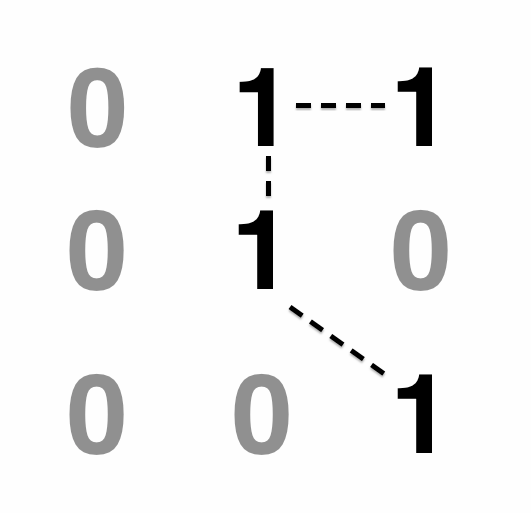
\includegraphics[width = 0.3\textwidth]{./images/m_adjacency}
  \end{minipage}
\end{description}

\subsubsection{Distance measures / Neighbors \buch{p.71}}
For pixels $p,q$  with coordinates $(x,y), (s,t)$
\paragraph{Euclidean}
\begin{equation}
D_e(p,q) = [(x-s)^2 + (y-t)^2]^{\frac{1}{2}}
\end{equation}
\paragraph{City-block}
\begin{equation}
D_4(p,q) = |x-s| + |y-t|
\end{equation}
Pixels with a $D_4 = 1$ are the 4-neighbors of $(x,y)$
\paragraph{Chessboard}
\begin{equation}
D_8(p,q) = max(|x-s|, |y-t|)
\end{equation}
Pixels with a $D_8 = 1$ are the 8-neighbors of $(x,y)$

\subsection{Math tools \buch{p.72}}
\subsubsection{Noise reduction \buch{p.75}}
Image with noise
\begin{equation}
g(x,y) = f(x,y) + \eta(x,y)
\end{equation}
Noise $\eta$ is uncorrelated and has zero average.  Averaging over $K$ different images reduces noise.
\begin{eqnarray}
\bar{g}(x,y)      =& \frac{1}{K} \sum\limits_{i=1}^{K}g_i(x,y) \notag \\
E\{\bar{g}(x,y)\}   =& f(x,y) \\ 
\sigma_{\bar{g}(x,y)}^2 =& \frac{1}{K} \sigma_{\eta(x,y)}^2 \notag
\end{eqnarray}

\subsubsection{Set and Logical Operations \buch{p.80}}
\begin{tabular}{|l|l|l|}
  \hline
  Subset			& $A \subseteq B$						& Every element of A is also in B
  \\ \hline
  Union			& $C = A \cup B$						& C contains all Elements in A, B or both
  \\ \hline
  Intersection	& $D = A \cap B$						& D contains all Elements wich are in A and B
  \\ \hline
  Complement		& $A^c = \{ \omega | \omega \in A\}$	& Set of elements that are not in A
  \\ \hline
  Difference		& $A-B = \{ \omega | \omega \in A, \omega \notin B\} = A \cap B^c$	&
  \\ \hline
\end{tabular}


\subsubsection{Neighborhood operations \buch{p.85}}
Averaging of neighborhood $S_{xy}$
\begin{equation}
g(x,y) = \frac{1}{mn} \sum_{(r,c)\in S_{xy}}f(r,c)
\end{equation}

\subsubsection{Geometric spatial Transformations \buch{p.87}}
\begin{minipage}{0.6\textwidth}
  \[
  (x,y) = T\{(v,w)\} \notag \\
  \]
  \[
  \text{affine transform:} \quad \left[ x~y~1 \right] = [ v~w~q ] \mathbf{T} = [ v~w~1 ] 
  \left[ \begin{array}{ccc}
  t_{11} & t_{12} & 0 \\
  t_{21} & t_{22} & 0 \\
  t_{31} & t_{32} & 1 \end{array} \right]
  \]
\end{minipage}
\begin{minipage}{0.4\textwidth}
  \begin{itemize}
\item Spatial transformation of coordinates
\item Intensity interpolation for transformed pixels
\item See p.88 for examples of $\mathbf{T}$!
\end{itemize}
\end{minipage}

\subsubsection{Image registration \buch{p.89}}
\begin{itemize}
  \item Tries to align several images of the same scheme
  \item Using \textbf{tie points}, whose location are known precisely
\end{itemize}


\section{Intensity Transformations and Spatial Filtering \buch{Chapter 3}}

\subsection{Basic intensity transformation functions}
\begin{equation}
s = T(r)
\end{equation}

\begin{itemize}
	\item Image negatives
		\begin{equation}
			s = L-1-r
		\end{equation}
	\item Log transformations
		\begin{equation}
			s = c \cdot \log{(1 + r)}
		\end{equation}
	\item Inverse log transformations
	\item Power-law (Gamma) transformations
		\begin{equation}
			s = c r^\gamma
		\end{equation}
	\item Piecewise-linear transformation functions
	\item Bit-plane slicing
		Split a image in slices for each intensity bit.  All resulting plane are binary images.
		May be used for a simple compression.
	
\end{itemize}


\subsection{Histogram processing}
The histogram shows the number of occurrence of a particular intensity level relative to the total number of pixels (probability of the intensity value)

\subsubsection{Histogram equalization}
The intensity level in an image may be viewed as random variables in the interval $[0, L-1]$.

\paragraph{For continuous Values}
\begin{equation}
	s = T(r) = (L-1)\int_0^r p_r(\omega) d\omega
\end{equation} 

\paragraph{For discrete Values}
\begin{equation}
	s_k = T(r_k) = (L-1) \sum_{j=0}^k p_r(r_j) = \frac{L-1}{MN} \sum_{j=0}^k n_j \qquad k = 0,1,2,\ldots, L-1
\end{equation}
where $MN$ is the total number of pixels, $n_k$ is the number of pixels that have the intensity $r_k$ and $L$ is the number of possible intensity levels in the image.
A plot of $p_r(r_k)$ versus $r_k$ is commonly referred to as a histogram.


\subsubsection{Histogram Matching (Specification)}
If we want to highlight only some intensity levels we need other methods than histogram equalization.

\paragraph{For continuous Values}
\begin{align}
	s	&= T(r) = (L-1) \int_0^r p_r(\omega) d\omega \label{eq:histmatch:cont1} \\
	G(z)&= (L-1) \int_0^z p_z(t) dt \label{eq:histmatch:cont2} \\
	z 	&= G^{-1}[T(r)] = G^{-1}(z) \label{eq:histmatch:cont3}
\end{align}

\begin{enumerate}
  \item Optain $p_r(r)$ from the original image and use Eq.\ref{eq:histmatch:cont1} to obtain the value of $s$.
  \item Use Eq.\ref{eq:histmatch:cont2} to obtain the transformation function $G(z)$
  \item Obtain the inverse transformation $z = G^{-1}(s)$
  \item Obtain the output image by first equalizing the original image using Eq.\ref{eq:histmatch:cont1}; the pixels values in this image are the $s$ values.
  	For each pixel witch value $s$ in the equalized image, perform the inverse mapping $z = G^{-1}(s)$ to obtain the corresponding pixel in the output image. 
\end{enumerate}

\paragraph{For discrete Values}
\begin{align}
	s_k		&= T(r_k) = \frac{L-1}{MN}\sum_{j=0}^{k} n_j \label{eq:histmatch:disc1} \\
	G(z_q)	&= (L-1) \sum_{i=0}^q p_z(z_i) = s_k \label{eq:histmatch:disc2}  \\
	z_q 	&= G^{-1}(s_k)	 
\end{align}

\begin{enumerate}
  \item Compute the histogram $p_r(r)$ of the given image.
  \item Find the histogram equalization transformation (Eq.\ref{eq:histmatch:disc1}), round the resulting $s_k$
  	values to the integer range $[o, L-1]$
  \item Compute all values of the transformation function $G$ using Eq.\ref{eq:histmatch:disc2}, where $p_z(z_i)$ are the values
  	of the specified histogram. Round the values of $G$ to integers and store them in a table
  \item For every value of $s_k$ use the stored values of $G$ to find the corresponding value of $z_q$ so that $G(z_q)$ is 
  	closest to $s_k$ and store these mappings from $s$ to $z$.
  \item Form the output image by first histogram-equalizing the input image and then mapping every equalized pixel value, $s_k$, of this
  	image to the corresponding value $z_q$ in the output image using the mappings found in step 4.
\end{enumerate}


\subsubsection{Local Histogram Processing}
The techniques described above are easily adapted to local enhancement. The procedure is to define a neighborhood and move its center from pixel to pixel.
At each location, the histogram of the neighborhood is computed and a transformation function is obtained. This function is then used to map the intensity
of the pixel centered in the neighborhood.


\subsubsection{Using Histogram Statistics for Image Enhancement}



\subsection{Fundamentals of spatial filtering\buch{p. 144}}
A spatial filter consist of
\begin{enumerate}
	\item neighborhood (typically a small rectangle)
	\item a predefined operation
\end{enumerate}
If the operation is linear its a \emph{linear spatial filter} otherwise its \emph{nonlinear}.
Linear filters may be described by a correlation or convolution of a filter $w(x,y)$ and the picture $f(x,y)$ 
\begin{eqnarray}
	\text{correlation:}& w(x,y) \text{\FiveStarOpen} f(x,y) = \sum\limits_{s=-a}^{a}\sum\limits_{t=-b}^{b}w(s,t) f(x+s, y+t) \\
	\text{convolution:}& w(x,y) \star f(x,y) = \sum\limits_{s=-a}^{a}\sum\limits_{t=-b}^{b}w(s,t) f(x-s, y-t) 
\end{eqnarray}
Correlation and convolution can be interchanged by rotating the filter by $180^\circ$.
% TODO: add picture
\subsubsection{Smoothing spatial filters}
The output of a smoothing, linear spatial filter is the average of the pixels contained in the neighborhood of the filter mask.
Its main application is blurring and thus reducing noise in images.
\begin{equation}
g(x,y) = \frac{\sum\limits_{s=-a}^{a}\sum\limits_{t=-b}^{b}w(s,t) f(x+s, y+t)}{\sum\limits_{s=-a}^{a}\sum\limits_{t=-b}^{b}w(s,t)}
\end{equation}
\paragraph{box filter}
A filter which all coefficients are equal:
$ \frac{1}{9} \cdot$ \begin{tabular}{|c|c|c|} \hline 1 & 1 & 1 \\ \hline 1 & 1 & 1 \\ \hline 1 & 1 & 1  \\ \hline \end{tabular}
\paragraph{weighted average}
Giving more importance to some pixels:
$ \frac{1}{16} \cdot$ \begin{tabular}{|c|c|c|} \hline 1 & 2 & 1 \\ \hline 2 & 4 & 2 \\ \hline 1 & 2 & 1  \\ \hline \end{tabular}
\subsubsection{Sharpening spatial filters}
This filter highlights transitions in intensity, thus sharpening the image.
It is the opposite of the smoothing filter and since they have a integrative effect it follows that sharpening filters have a derivative effect.
\begin{align}
\frac{\partial f}{\partial x} &= f(x+1) - f(x)& \text{first order derivative} \\
\frac{\partial^2 f}{\partial x^2} &= f(x+1) + f(x-1)  -2 f(x)& \text{second order derivative}
\end{align}

\paragraph{Second Derivative - Laplacian}
The Laplacian is a isotropic (rotation invariant) derivative operator
\begin{align}
\nabla^2f &= \frac{\partial^2 f}{\partial x^2} + \frac{\partial^2 f}{\partial y^2} \\
\nabla^2f &= f(x+1,y) + f(x-1,y) + f(x,y+1) + f(x,y-1) - 4 f(x,y)
\end{align}

\begin{tabular}{|c|c|c|} \hline
0 & 1 & 0  \\ \hline
1 &-4 & 1  \\ \hline
0 & 1 & 0  \\ \hline
\end{tabular}
Implementation with filter masks (rotation invariant for $90^\circ$ rotations)

\begin{tabular}{|c|c|c|} \hline
1 & 1 & 1 \\ \hline
1 &-8 & 1 \\ \hline
1 & 1 & 1 \\ \hline
\end{tabular}
Incorporating the diagonal directions (rotation invariant for $45^\circ$ rotations)
\\ \\
To sharpen an image we add the Laplacian to the original

\begin{equation}
g(x,y) = f(x,y) + c \left[ \nabla^2f(x,y) \right]
\end{equation}

\paragraph{Unsharp Masking / Highboost}
\begin{enumerate}
\item Blur the original $\bar{f}$
\item Subtract the blurred image from the original (gives the mask $g_{mask}$)
\item Add the mask to the original
\end{enumerate}
\begin{align}
g_{mask}(x,y) &= f(x,y) - \bar{f}(x,y) \\
g(x,y) &= f(x,y) + k \cdot g_{mask}(x,y)
\end{align}

with $k=1$ this filter is called unsharp masking, with $k>1$ highboost.

\paragraph{First-Order Derivative - Gradient}
The first derivative in an image is the magnitude of the gradient.
The gradient of image $f$ at $(x,y)$ is a two-dimensional \emph{vector} pointing in the direction of the greatest rate of change.
\begin{equation}
\nabla f \equiv grad(f) \equiv \begin{pmatrix}g_x\\g_y\end{pmatrix} = \begin{pmatrix} \dfrac{\partial f}{\partial x} \\ \\ \dfrac{\partial f}{\partial y} \end{pmatrix}
\end{equation}
The magnitude of the gradient, is the value of the rate of change into the direction of the gradient.
\begin{equation}
M(x,y) = \sqrt{g_x^2 + g_y^2}
\end{equation}
\begin{itemize}
\item isotropic but not linear
\item $M(x,y)$ is called the gradient image
\item a popular approximation is $M(x,y) \approx |g_x| + |g_y|$
\end{itemize}

The gradient can be approximated using filter masks.

\begin{itemize}
	\item Roberts cross gradient operators
		\begin{itemize}
		\item \begin{tabular}{|c|c|} \hline
		-1 & 0 \\ \hline
		 0 & 1 \\ \hline
		\end{tabular}
		\begin{tabular}{|c|c|} \hline
		 0 &-1 \\ \hline
		 1 & 0 \\ \hline
		\end{tabular}
	\item no center of symmetry $\rightarrow$ difficult to implement
	\end{itemize}
		\item  Sobel operators
		\begin{itemize}
		\item \begin{tabular}{|c|c|c|} \hline
		-1 &-2 &-1 \\ \hline
		 0 & 0 & 0 \\ \hline
		 1 & 2 & 1 \\ \hline
		\end{tabular}
		\begin{tabular}{|c|c|c|} \hline
		-1 & 0 & 1 \\ \hline
		-2 & 0 & 2 \\ \hline
		-1 & 0 & 1 \\ \hline
		\end{tabular}
		\item 3x3 neighborhood $\rightarrow$ smoothing
		\end{itemize}
\end{itemize}

\newpage
\section{Filtering in the frequency domain \buch{p.199}}
\subsection{Countinous Fourier Transform \buch{p.205}}
\subsection{Sampling \buch{p.211}}
Multiplication of the function with an impulse train
\begin{equation}
\tilde{f}(t) = f(t) s_{\Delta T}(t) = \sum_{n=-\infty}^{\infty}f(t)\sigma (t-n \Delta T)
\end{equation}
The fourier transform of it
\begin{equation}
\tilde{F}(\mu) = F(\mu) \star S(\mu) = \frac{1}{\Delta T} \sum_{n=-\infty}^{\infty}F\left(\mu - \frac{n}{\Delta T}\right)
\end{equation}

\subsection{The discrete Fourier transform of one variable \buch{p.220}}
The Fourier transform of sampled data is continuous and infinitely periodic with period $1/\Delta T$
\begin{equation}
\tilde{F}(\mu)= \sum_{n=-\infty}^{\infty} f_n \cdot e^{-j 2 \pi  \mu n \Delta T}
\end{equation}

We are only interested in one period.
So we obtain $M$ equally spaced samples of $\tilde{F}(\mu)$ over the period $\mu = 0$ to $\mu = 1/\Delta T$
\begin{equation}
\mu = \frac{m}{M \Delta T}
\end{equation}

This results in

\begin{equation}
F_m = \sum_{n=0}^{M-1} f_n \cdot e^{-j 2 \pi m n / M} \quad m = 0,1,2,\dots,M-1
\end{equation}
 
The \emph{inverse discrete Fourier transform} is used to recover the sample set ${f_n}$
\begin{equation}
f_n = \frac{1}{M} \sum_{m=0}^{M-1}F_m e^{j 2 \pi m n / M} \quad n = 0,1,2,\dots,M-1
\end{equation}

\begin{itemize}
\item The discrete Fourier transform is an invertible, linear transformation
\item The DFT pair is applicable to \emph{any} finite set of uniformly discrete samples
\item DFT and IDFT are periodic with period M
\end{itemize}
 
\subsubsection{Sampling and Frequency Intervals \buch{p.223}}
If $f(x)$ consists of $M$ samples, taken $\Delta T$ units apart, the duration $T$ of the record is
\begin{equation}
	T = M \Delta T
\end{equation}
The corresponding spacing in the discrete frequency domain $\Delta u$ is
\begin{equation}
	\Delta u = \frac{1}{M \Delta T} = \frac{1}{T}
\end{equation}
The frequency range spanned by the $M$ components of the DFT is
\begin{equation}
	\Omega = M \Delta u = \frac{1}{\Delta T}
\end{equation} 

\subsection{2D Countinous FT \buch{p.205}} 
\subsection{The 2D Impulse \buch{p.225}}
The discrete 2D impulse is defined as
\begin{equation}
\delta(x,y) = 
\begin{cases} 1 & \text{if $x=y=0$,}
\\
0 &\text{otherwise}
\end{cases}
\end{equation}

with the sifting property
\begin{equation}
\sum_{x=-\infty}^{\infty}\sum_{y=-\infty}^{\infty}f(x,y) \delta(x,y) = f(0,0)
\end{equation}

\subsection{2D Sampling Theorem}
A continuous, band-limited function $f(t,z)$ can be recovered with no error if the sampling intervals are\\
 \begin{minipage}{0.4\textwidth}
   \[
   \Delta T < \dfrac{1}{2 u_{max}}
   \]
 \end{minipage} 
and
  \begin{minipage}{0.4\textwidth}
    \[
    \Delta Z < \dfrac{1}{2 v_{max}}
    \]
  \end{minipage} 
  
  

\subsection{2D DFT and IDFT \buch{p.235}}

\subsubsection{2D DFT}
\begin{equation}
    F(u,v) = \sum_{x=0}^{M-1}\sum_{y=0}^{N-1}f(x,y)\cdot e^{-j2\pi \left(\frac{ux}{M}+ \frac{vy}{N}\right)}
\end{equation}
\begin{center}
  with $u$ and $v$ in the ranges $u = 0,1,2,\ldots,M-1$ and $v = 0,1,2,\ldots,N-1$
\end{center}
\subsubsection{2D IDFT}
\begin{equation}
    f(x,y) = \frac{1}{MN} \sum_{u=0}^{M-1}\sum_{v=0}^{N-1}F(u,v)\cdot e^{j2\pi \left(\frac{ux}{M}+ \frac{vy}{N}\right)}
\end{equation}
\begin{center}
  with $x$ and $y$ in the ranges $x = 0,1,2,\ldots,M-1$ and $y = 0,1,2,\ldots,N-1$
\end{center}

\subsubsection{Properties}
\begin{itemize}
\item Separation between samples in the frequency domain are inversely proportional to the spacing between spatial samples and the number of samples
$\Delta u = \frac{1}{M \Delta T} \quad \Delta v = \frac{1}{N \Delta Z}$
\item Infinitely periodic
\item Symmetry properties \buch{p.242}, see Table \ref{tab:Symmetry_2D_DFT} (Appendix)
\item Summary of properties \buch{p.253}, see Table \ref{tab:Properties_2D_DFT} and \ref{tab:DFT_Pairs} (Appendix)
\end{itemize}

\subsubsection{Periodicity \buch{237}}
  Visualization is simplified if we shift the data so that F(0,0) at (M/2,N/2) with
    \begin{equation}
      f(x,y)(-1)^{x+y} \Leftrightarrow F(u-M/2, v-N/2)
    \end{equation}
    
\subsubsection{"DC"}
  \begin{equation}
    |F(0,0)| = MN|\bar{f}(x,y)|
  \end{equation}

\subsubsection{2-D Convolution \buch{p.249}}
The 2-D Convolution Theorem is given by:
\begin{align}
	f(x,y) \bigstar h(x,y) \Leftrightarrow F(u,v)H(u,v)
\end{align}

It is necessairy to zero-pad the images $f(x,y)$ of size $A \times B$ and $h(x,y)$ of size $C \times D$ as follows:

\begin{equation}
	f_p(x,y) = 
		\begin{cases} 
			f(x,y) & 0 \leq x \leq A-1 \text{  and  } 0 \leq y \leq B-1 \\
			0 & A \leq x \leq P \text{  or  } B \leq y \leq Q
		\end{cases}
\end{equation}
\begin{equation}
	h_p(x,y) = 
		\begin{cases}
			h(x,y) & 0 \leq x \leq C-1 \text{  and  } 0 \leq y \leq D-1 \\
			0 & C \leq x \leq P \text{  or  } D \leq y \leq Q
		\end{cases}
\end{equation}
with
\begin{align}
	P &\geq A+C-1 \\
	Q &\geq B+D-1
	\label{equ:2D_Conv_Padding}
\end{align}
resulting in padded images of size $P \times Q$

\subsection{Basics of Filtering in the Frequency Domains}
  Generally, filtering in the frequency domain is obtained by
  \begin{equation}
  g(x,y) = \Im^{-1} \left[ H(u,v) F(u,v) \right]
  \end{equation}
  if filter $H(u,v)$ is real \& symmetric
  \begin{equation}
  g(x,y) = \Im^{-1} \left[ H(u,v) \cdot R(u,v) + j H(u,v) \cdot I(u,v)\right]
  \end{equation}  
  $\Rightarrow$ Filter that affect real and imaginary parts equally have no effect on the phase $\rightarrow$ \textbf{zero-phase-shift} filters 

\subsubsection{Summary of Steps for Filtering in the Frequency Domain \buch{p.263}}
  
\begin{enumerate}
	\item Given an input image $f(x,y)$ of size $M \times N$, obtain the padding parameters $P$ and $Q$ from Eq. \ref{equ:2D_Conv_Padding}. Typically, we select $P=2M$ and $Q=2N$.
	\item Form a padded image, $f_p(x,y)$, of size $P \times Q$ by appending the necessary number of zeros to $f(x,y)$.
	\item Multiply $f_p(x,y)$ by $(-1)^{x+y}$ to center its transform.
	\item Compute the DFT, $F(u,v)$, of the image from step 3.
	\item Generate a real, symmetric filter function, $H(u,v)$, of size $P \times Q$ with center at coordinates $(P/2,Q/2)$. Form the product $G(u,v) = H(u,v) F(u,v)$ using array multiplication.
	\item Obtain the processed image, $g_p(x,y) = \left\lbrace \text{real} \left[ \Im^{-1} \left[ G(u,v) \right] \right] \right\rbrace (-1)^{x+y}$, where the real part is selected in order to ignore parasitic complex components resulting from computational inaccuracies, and the subscript $p$ indicates that we are dealing with padded arrays.
	\item Obtain the final processed result, $g(x,y)$, by extracting the $M \times N$ region from the top, left quadrant of $g_p(x,y)$.
\end{enumerate}

\subsection{Image smoothing using frequency domain filters \buch{p.269}}
\subsubsection{Ideal Lowpass Filters}
\begin{equation}
	H(u,v)  = 
		\begin{cases}
			1 & \text{  if } D(u,v) \leq D_0 \\
			0 & \text{  if } D(u,v) > D_0 \\ 
		\end{cases}
\end{equation}
where $D_0$ is a positive constant and $D(u,v)$ is the distance between a point $(u,v)$ in the frequency domain and the center of the frequency rectangle; that is,
\begin{equation}
	D(u,v) = \left[ (u-P/2)^2 + (v-Q/2)^2 \right]^{1/2}
	\label{equ:Freq_Filter_D_uv}
\end{equation}
ILPFs have a \textbf{huge ringing problem} and are not frequently used.

\subsubsection{Butterworth Lowpass Filters}
The transfer function of a Butterworth lowpass filter (BLPF) of order $n$, and with cutoff frequency at a distance $D_0$ from the origin, is defined as
\begin{equation}
	H(u,v) = \frac{1}{1 + \left[ D(u,v) / D_0 \right]^{2n}}
\end{equation}
The BLPF of order 1 has no ringing, but ringing can become significant in filters of higher order. Usually only BLPFs with $n \leq 4$ are used.

\subsubsection{Gaussian Lowpass Filters}
A Gaussian lowpass filter (GLPF) of two dimensions is given by
\begin{equation}
	H(u,v) = e^{-D^2(u,v)/2D_0^2}
\end{equation}
where $D_0$ is the cutoff frequency. When $D(u,v)=D_0$, the GLPF is down to $0.607$ of its maximum value. The GLPF will have \textbf{no ringing}.

\subsection{Image sharpening using frequency domain filters \buch{p.280}}
A highpass filter is obtained from a given lowpass filter by
\begin{equation}
	H_{HP}(u,v) = 1 - H_{LP}(u,v)
\end{equation}

\subsubsection{Ideal Highpass Filters}
A ideal highpass filter (IHPF) is defined as
\begin{equation}
	H(u,v) = 
		\begin{cases}
			0 & \text{  if } D(u,v) \leq D_0 \\
			1 & \text{  if } D(u,v) > D_0
		\end{cases}
\end{equation}
where $D_0$ is the cutoff frequency and $D(u,v)$ is given by Eq. \ref{equ:Freq_Filter_D_uv}. Like the ILPF, the IHPF creates a large ringing.

\subsubsection{Butterworth Highpass Filters}
A 2-D Butterworth highpass filter (HBPF) of order $n$ and cutoff frequency $D_0$ is defined as 
\begin{equation}
	H(u,v) = \frac{1}{1 + \left[ D_0 / D(u,v) \right]^{2n}}
\end{equation}

\subsubsection{Gaussian Highpass Filters}
The transfer function of the Gaussian highpass filter (GHPF) with cutoff frequency at $D_0$ is given by
\begin{equation}
	H(u,v) = 1 - e^{-D^2(u,v)/2D_0^2}
\end{equation}

\subsubsection{The Laplacian in the Frequency Domain \buch{p.286}}
The Laplacian can be implemented in the frequency domain using the filter
\begin{equation}
	H(u,v) = -4 \pi^2 D^2(u,v)
	\label{equ:Laplacian_Freq_Domain}
\end{equation}
The Laplacian image is obtained as
\begin{equation}
	\nabla^2 f(x,y) = \Im^{-1} \left\lbrace H(u,v)F(u,v) \right\rbrace 
	\label{equ:laplacian_freq_backtransform}
\end{equation}

The enhanced image $g(x,y) = f(x,y) + c \nabla^2f(x,y)$ with $c=-1$ can be achieved by
\begin{equation}
	g(x,y) = \Im^{-1} \left\lbrace \left[ 1 + 4 \pi^2 D^2(u,v) \right] F(u,v) \right\rbrace 
\end{equation}

Usually, $f(x,y)$ is normalized to the range $\left[0,1\right]$ and $\nabla^2 f(x,y)$ is divided by its maximum value, which brings it to the approximate range $\left[-1,1\right]$. The normalizing factor in the frequency domain is not easily computed, so the preferred frequency domain implementation is using the equation
	\begin{equation}
		g(x,y) = f(x,y) + c \nabla^2f(x,y)
	\end{equation}
with $\nabla^2f(x,y)$ computed using Eq.  \ref{equ:laplacian_freq_backtransform}.

\subsubsection{Unsharp Masking, Highboost Filtering, and High-Frequency-Emphasis Filtering \buch{p.288}}
A high-frequency-emphasis filter is achieved by
\begin{equation}
	g(x,y) = \Im^{-1} \left\lbrace \left[ k_1 + k_2 \cdot H_{HP}(u,v) \right] F(u,v) \right\rbrace 
\end{equation}
where $k_1 \geq 0$ gives control of the offset from the origin and $k_2 \geq 0$ controlls the contribution of high frequencies.

\subsubsection{Homomorphic Filtering \buch{p.290}}
\begin{minipage}{9cm}
	Homomorphic filtering is used to separate illumination and reflectance components. This is achieved by using the natural logarithm $\ln$ before applying the DFT.
\end{minipage}
\begin{minipage}{9cm}
	\adjustbox{width=9cm}{\begin{tikzpicture}
\tikzstyle{gray_block} = [draw,outer sep=0,inner sep=5,minimum size=50,line width=1, very thick, draw=black!55, top color=white,bottom color=black!20]
\tikzstyle{vecArrow} = [thick, decoration={markings,mark=at position
   1 with {\arrow[semithick]{open triangle 60}}},
   double distance=1.4pt, shorten >= 5.5pt,
   preaction = {decorate},
   postaction = {draw,line width=1.4pt, white,shorten >= 4.5pt}]
   
	\node (a) at (-2.2,0) {$f(x,y)$};
    \node (b) [gray_block] at (0,0) {ln};
	\node (c) [gray_block] at (2.2,0) {DFT};
	\node (d) [gray_block] at (4.4,0) {$H(u,v)$};
	\node (e) [gray_block] at (6.6,0) {(DFT)$^{-1}$};
	\node (f) [gray_block] at (8.8,0) {exp};
	\node (g) at (11,0) {$g(x,y)$};
	
	\draw[vecArrow] (a) node[right] {} -> (b) node [left] {};
	\draw[vecArrow] (b) node[right] {} -> (c) node [left] {};
	\draw[vecArrow] (c) node[right] {} -> (d) node [left] {};
	\draw[vecArrow] (d) node[right] {} -> (e) node [left] {};
	\draw[vecArrow] (e) node[right] {} -> (f) node [left] {};
	\draw[vecArrow] (f) node[right] {} -> (g) node [left] {};
	
\end{tikzpicture}}
\end{minipage} \\

A modified version of a Gaussian highpass,
\begin{equation}
	H(u,v) = (\gamma_H - \gamma_L) \left[ 1 - e^{-c \left[ D^2(u,v) / D_0^2 \right]} \right] + \gamma_L
\end{equation}
allows to attenuate the low frequencies (illumination) with $\gamma_L < 1$ and amplify the high frequencies (reflectance) with $\gamma_H > 1$.

\newpage
\subsection{Selective Filtering \buch{p.294}}

\subsubsection{Bandreject and Bandpass Filters} \label{subsubsec:FilteringFrequency_BandrejectFilters}
Bandreject filters are given by the following equations,

\begin{table}[htbp]
	\centering
	\begin{tabular}{|ccc|}
		\hline
		\textbf{Ideal} & \textbf{Butterworth} & \textbf{Gaussian} \\ \hline
		$H(u,v) = 
			\begin{cases}
				0 & \text{  if } D_0-\frac{W}{2} \leq D \leq D_0 + \frac{W}{2} \\
				1 & \text{  otherwise}
			\end{cases} $
		& $H(u,v) = \frac{1}{1 + \left[ \frac{DW}{D^2 - D_0^2} \right]^{2n}}$
		& $H(u,v) = 1-e^{-\left[\frac{D^2-D_0^2}{DW}\right]^2}$ \\
		\hline
	\end{tabular}
\end{table}

where $D_0$ is the radial center of the band, $W$ is the width of the band, and $D(u,v)$ is given by Eq. \ref{equ:Freq_Filter_D_uv}. \\

A bandpass filter is obtained by
\begin{equation}
	H_{BP}(u,v) = 1 - H_{BR}(u,v)
\end{equation}

\subsubsection{Notch Filters}  \label{subsubsec:FilteringFrequency_NotchFilters}
A notch filter rejects (or passes) frequencies in a predefined neighborhood about the center of the frequency rectangle. Notch reject filters are constructed as products of highpass filters whose centers have been translated to the centers of the notches. The general form is
\begin{equation}
	H_{NR}(u,v) = \prod_{k=1}^{Q} H_k(u,v) H_{-k}(u,v)
\end{equation}
where $H_k(u,v$ and $H_{-k}(u,v)$ are highpass filters whose centers are at $(u_k,v_k)$ and $(-u_k,-v_k)$. \\

A notch pass filter is obtained from a notch reject filter by
\begin{equation}
	H_{NP}(u,v) = 1 - H_{NR}(u,v)
\end{equation}

\subsection{Implementation \buch{p.298}}
\newpage
\section{Image restoration and reconstruction \buch{p.311}}
\subsection{Noise models  \buch{p.313}}

\subsection{Restoration in the presence of noise only - spatial filtering \buch{p.322}}
\subsubsection{Mean Filters}

\textbf{Arithmetic mean filter}\\
This filter is a standard filter.
\begin{equation}
	\hat{f}(x,y)= \frac{1}{m  n} \sum\limits_{(s,t)\in S_{xy}}g(s,t)
\end{equation}

\textbf{Geometric mean filter}\\
Smooth similar to arithmetic mean, but less loss of detail.
\begin{equation}
	\hat{f}(x,y)= \left[\prod\limits_{(s,t)\in S_{xy}} g(s,t)\right]^\frac{1}{mn}
\end{equation}

\textbf{Harmonic mean filter}\\
Works well on slat noise and not work for pepper noise. It does well also with other types of noise like Gaussian noise
\begin{equation}
	\hat{f}(x,y)= \frac{mn}{\sum\limits_{(s,t)\in S_{xy}} \frac{1}{g(s,t)}}
\end{equation}

\textbf{Contraharmonic mean filter}\\
\begin{itemize}
\item For positive Q, good for pepper noise
\item For negative Q, good for salt noise
\item For Q = -1, it is a harmonic mean filter
\item For Q = 0, it is a arithmetic mean filter\\ \\
\textbf{This filter can not simultaneously reduce salt and pepper noise}
\end{itemize}

\begin{equation}
	\hat{f}(x,y)= \frac{\sum\limits_{(s,t)\in S_{xy}} g(s,t)^{Q+1}}{\sum\limits_{(s,t)\in S_{xy}} g(s,t)^Q}
\end{equation}

\subsubsection{Order-Statistic Filters \buch{p.325}}

The output of these filters depends on the order of the pixel values. \\ \\

\textbf{Median filter}\\
Quite popular, since they result in good noise, without much smoothing \\
\begin{equation}
	\hat{f}(x,y)=\underset{(s,t) \in S_{xy}}{\text{median}}\{g(s,t) \}
\end{equation}

\textbf{Max filter}\\
This filter picks the maximum of the neighborhood, also it reduce the pepper noise.
\begin{equation}
	\hat{f}(x,y)=\underset{(s,t) \in S_{xy}}{\text{max}}\{g(s,t) \}
\end{equation}

\textbf{Min filter}\\
This filter picks the minimum of the neighborhood, also it reduce the salt noise.
\begin{equation}
	\hat{f}(x,y)=\underset{(s,t) \in S_{xy}}{\text{min}}\{g(s,t) \}
\end{equation}

\textbf{Midpoint filter}\\
The midpoint filter simply computes the midpoint between the maximum and the minimum values in the neighborhood. \\
It works best for randomly distributed noise, like Gaussian or uniform noise.
\begin{equation}
	\hat{f}(x,y)=\frac{1}{2} \left[ \underset{(s,t) \in S_{xy}}{\text{max}}\{g(s,t) \} + \underset{(s,t) \in S_{xy}}{\text{min}}\{g(s,t) \}\right]
\end{equation}

\textbf{Alpha-trimmed filter}\\
It is robust against outliers and it is good against "normal" noise.\\ 

Suppose that we delete the $d/2$ lowest and $d/2$ highest intensity values of $g(s,t)$ in the neighborhood $S_{xy}$. Let $g_r{s,t}$ represent the remaining $mn-d$ pixels.
\begin{itemize}
	\item $d$ can range from $mn-1$
	\item When $d=0$, then it is a arithmetic mean filter
	\item When $d=mn-1$, then the filter becomes a median filter
\end{itemize}
\begin{equation}
	\hat{f}(x,y)=\frac{1}{mn-d} \sum\limits_{(s,t)\in S_{xy}} g_r(s,t)
\end{equation}
\newpage

\subsubsection{Adaptive Filter \buch{p.330}}
Change the filter, depending on the contents of $S_{xy}$
\begin{itemize}
	\item The local mean $m_L$ and the local variance $\sigma_{L}^2$ can be used as compact descriptors of $S_{xy}$
	\item The ration of the variances can in theory never be lager then 1
	\item In practice, since the noise variance $\sigma_{\eta}^2$ needs to be estimated (schätzen), this must be enforced.
	\item $\sigma_{\eta}^2 \le \sigma_{L}^2$
\end{itemize}

\begin{equation}
	\hat{f}(x,y)=g(x,y) - \frac{\sigma_{\eta}^2}{\sigma_{L}^2} \left[g(x,y)-m_L \right]
\end{equation}

\subsubsection{Notch Filter \buch{p.337}}
\subsection{Restoration in the presence of noise only - frequency domain filtering for periodic noise \buch{p.335}}


\subsection{Estimating the degradation function \buch{p.346}}


\subsection{Inverse filtering \buch{p.351}}

\begin{itemize}
	\item Clearly, even though we might know $H(u,v)$ perfectly, the noise makes it impossible to recover $f(x,y)$
	\item Furthermonre, if H(u,v) is close to zero, $\frac{N(u,v)}{H(u,v)}$ will dominate the result, rendering it useless.
	\item One trick is, to focus on $H(u,v)$ near the origin, where it tends to be lager.
\end{itemize}

\begin{equation}
	\hat{F}(x,y)= F(u,v) + \frac{N(u,v)}{H(u,v)}
\end{equation}


\subsection{Minimum Mean Square Error Filtering (Wiener) \buch{p.352}}
\subsection{Constrained least squares filtering \buch{p.357}}


\subsection{Geometric mean filter \buch{p.361}}



\newpage
\section{Color image processing \buch{p.394}}
\subsection{Color fundamentals \buch{p.395}}
\begin{itemize}
	\item Humans can perceive thousands of colors but only about 20-30 shades of gray
	\item Color is often a great feature of object detection and extraction
	\item White light can be split into a spectrum of colors
	\item The human visual system (HVS) is quite complex, but basically, the cones are responsible for the color vision
	\begin{itemize}
		\item There are about 7 million cones which can be put into three categories
		\begin{itemize}
			\item $65\% $ are sensitive to red
			\item $33\% $ are sensitive to green
			\item $2\% $ are sensitive to blue
		\end{itemize}
		\item while their numbers vary widely, their sensitivity is quite similar
		\begin{itemize}
			\item Therefore, the blue cones are the most sensitive
			\item But the spatial resolution of red is much higher than that of blue
		\end{itemize}
	\end{itemize}
	\item Red, Green and Blue are called additive primary colors
	\item Magenta, Yellow and Cyan are called subtractive primary colors
	\item Humans often describe color using
	\begin{description}
		\item[Brightness:] Chromatic notation of intensity
		\item[Hue:] The dominant color
		\item[Saturation:] How much white light is mixed in with the pure color
	\end{description}
	\item The very useful HIS (Hue, Saturation, Intensity) color space is based on the color perception of humans	
\end{itemize}

The amount of red(X), green (Y) and blue (Z) needed to form a given color are called the tristimulus values.
A color can then be specified using its trichromatic coefficients x,y and z, which are normalized so that they sum to 1.
For any wavelength of light in the visible spectrum, these values can be read from tables that are the results from extensive experimentation.

\[
	x = \frac{X}{X+Y+Z} \qquad
	y = \frac{Y}{X+Y+Z} \qquad
	z = \frac{Z}{X+Y+Z}
\]



\subsection{Color models \buch{p.401}}
A color model is also called a color space or a color system. It allows colors to be represented in a well defined way, and depending on the task at hand, one model might be better suited than another.

\subsubsection{RGB model \buch{p.402}}
Based on the three primary colors of the HVS and the most used model as most color camera systems and monitors have these three channels.


\subsubsection{CMY and CMYK model \buch{p.406}}
These are models well suited for the primary colors of pigments, such as used in printing. The K stands for black, which, in theory can be mixed by summing up all subtractive primary colors, but for printing, the result tends to be a bit muddy, hence black is its own color. \\

If all color values have been normalized, the conversion from an RGB to a CMY image is achieved by
\begin{equation}
	\left[ \begin{array}{l} C \\ M \\ Y \end{array} \right] = \left[ \begin{array}{l} 1 \\ 1 \\ 1 \end{array} \right] - \left[ \begin{array}{l} R \\ G \\ B \end{array} \right]
\end{equation}

\subsubsection{The HSI Color Model \buch{p.407}}
The HSI Color Model is well suited for image processing algorithms.\\
\begin{minipage}{0.6\textwidth}
\begin{itemize}
	\item \textbf{H} - hue: information about color, determined by an angle from some reference point $\rightarrow$ usually an angle of $0^\circ$ at the red axis.
	\item \textbf{S} - saturation: length from the origin to the arbitrary color point
	\item \textbf{I} - intensity: given by the position of the plane on the vertical intensity axis.
\end{itemize}
\end{minipage}
\hspace{0.05\textwidth}
\begin{minipage}{0.35\textwidth}
	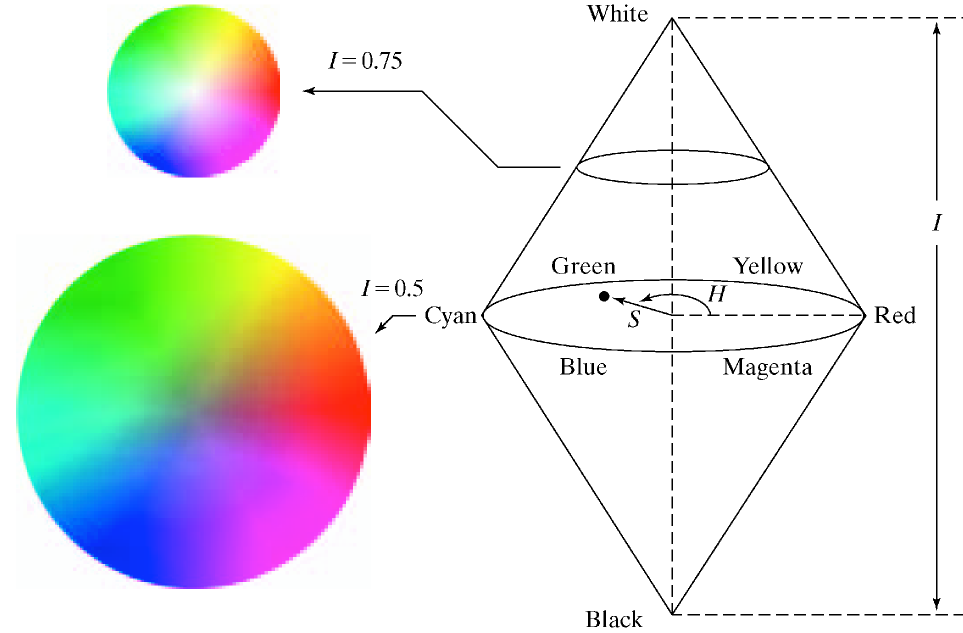
\includegraphics[width = \textwidth]{./images/HSI_ColorSpace}
\end{minipage}

\subsubsection{Converting RGB $\Rightarrow$ HSI \buch{p.410}}
The $H$ component of each RGB pixel is obtained by
\begin{equation}
	H = \begin{cases}
			\theta & \text{ if } B \leq G \\
			360 - \theta & \text{ if } B > G
		\end{cases}
\end{equation}
with
\begin{equation}
	\theta = \cos^{-1} \left[ \frac{\frac{1}{2} \left[ (R-G) + (R-B) \right]}{\left[(R-G)^2 + (R-B)(G-B)\right]^{1/2}} \right]
\end{equation}

The saturation component is given by
\begin{equation}
	S = 1 - \frac{3}{(R+G+B)} \left[ \min(R,G,B) \right]
\end{equation}

The intensity component is given by
\begin{equation}
	I = \frac{1}{3}(R+G+B)
\end{equation}

\subsubsection{Converting HSI $\Rightarrow$ RGB \buch{p.411}}
Given values of HSI in the interval $[0,1]$, the applicable equations depend on the values of $H$, according to the $120^{\circ}$ intervals separating the primaries.\\

First, $H$ is multiplied by $360^{\circ}$ so its range is $[0^{\circ},360^{\circ}]$. \\

\begin{tabularx}{\linewidth}{|l|X|X|X|}
	\hline 
	& \textbf{RG sector} ($0^{\circ} \leq H < 120^{\circ}$) & \textbf{GB sector} ($120^{\circ} \leq H < 240^{\circ}$) & \textbf{BR sector} ($240^{\circ} \leq H < 360^{\circ}$) \\ \hline
	$\mathbf{H}$ & $H = H$ & $H = H-120^{\circ}$ & $H = H-240^{\circ}$ \\ \hline
	$\mathbf{R}$ & $R = I \left[ 1 + \frac{S \cos(H)}{\cos(60^{\circ} - H)} \right]$ & $R = I(1-S)$ & $R = 3I - (R+B)$ \\
	$\mathbf{G}$ & $G = 3I - (R+B)$ & $G = I \left[ 1 + \frac{S \cos(H)}{\cos(60^{\circ} - H)} \right]$ & $G = I(1-S)$ \\
	$\mathbf{B}$ & $B = I(1-S)$ & $B = 3I - (R+B)$ & $B = I \left[ 1 + \frac{S \cos(H)}{\cos(60^{\circ} - H)} \right]$ \\
	\hline
\end{tabularx}


\subsection{Pseudo color image processing \buch{p.414}}
\begin{itemize}
	\item Assigning colors to gray values, based on a specified criterion.
	\item Goal: better human visualization and interpretation. \\
			Reason: humans can perceive thousands of color shades, but only 20-30 shades of gray.
\end{itemize}

\subsubsection{Intensity Slicing \buch{p.415}}
A gray-scale image with $[0,L-1]$ values is sliced into $P$ planes at the intensity levels $l_1,l_2,\dots,l_P$, creating the $P+1$ intervals $V_1,V_2,\dots,V_{P+1}$. Intensity to color assignments are made according to
\begin{equation}
	f(x,y) = c_k \qquad \qquad \text{if } f(x,y) \in V_k
\end{equation}
where $c_k$ is the color associated with the $k$th intensity interval $V_k$.

\subsubsection{Intensity to color transformation \buch{p.418}}
\begin{minipage}{12cm}
	A more general way than image slicing is to perform three independent transformations on the intensity. This method produces an image, whose color content is modulated by the transformation functions, which are only dependent on the intensity values.
\end{minipage}
\begin{minipage}{6cm}
	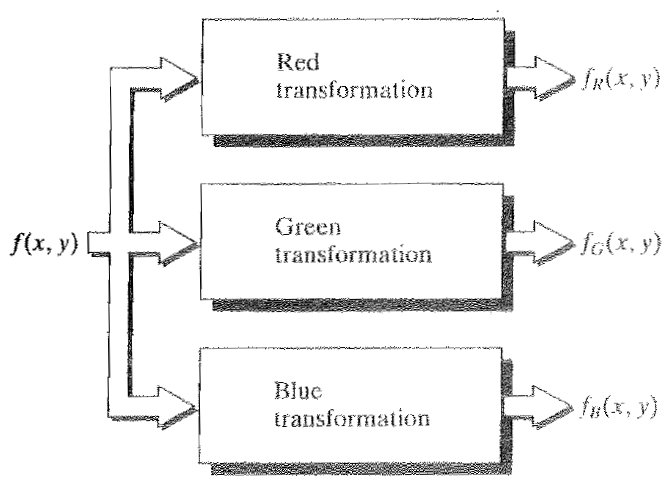
\includegraphics[width=6cm]{images/Pseudocolor_Processing.png}
	%TODO: unbedingt vertikzisieren!!!
\end{minipage}

\subsection{Full-Color Image Processing \buch{p.424}}
In the RGB system, each point is represented by a vector
\begin{equation}
	c = \left[\begin{array}{l}
		c_R \\ c_G \\ c_B
	\end{array} \right]
	= \left[\begin{array}{l}
		R \\ G \\ B
	\end{array} \right]
	\qquad \text{thus an image is represented by} \qquad
	c(x,y) = \left[\begin{array}{l}
		c_R(x,y) \\ c_G(x,y) \\ c_B(x,y)
	\end{array} \right]
	= \left[\begin{array}{l}
		R(x,y) \\ G(x,y) \\ B(x,y)
	\end{array} \right]	
\end{equation}

\subsection{Color Transformations \buch{p.426}}
Color transformations describe processing of a color image within a \textit{single} color model. Any transformation can be performed in any color model, howere some operations are better suited to specific models. \\

Generally a transformation is described by 
\begin{equation}
	g(x,y) = T\left[f(x,y)\right]
\end{equation}
where $T$ is an operator on $f$ over a spatial neighborhood. Each pixel value is a triplet or quartet. \\

\subsubsection{Color complements \buch{p.430}}
\begin{minipage}{12cm}
	The hues directly opposite one another are called \textit{complements}. They are analogous to the gray-scale negatives and are useful for enhancing details. The transformations can be achieved in the RGB or the HSI color spaces using the transfer functions shown on the right.
\end{minipage}
\begin{minipage}{6cm}
	\centering
	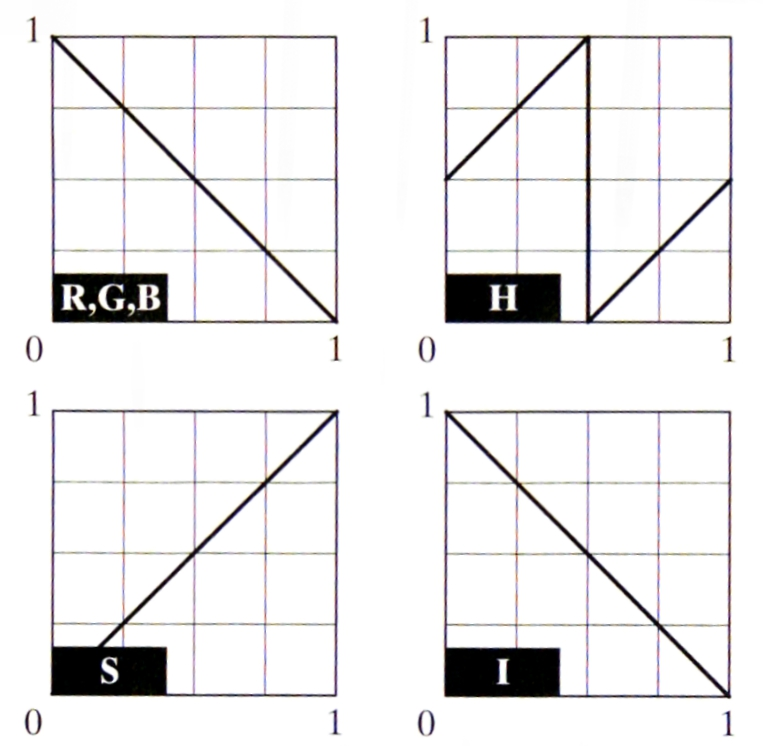
\includegraphics[width=4cm]{images/ColorComplements.jpeg}
	%TODO: vertikzisieren und evtl. anders anordnen
\end{minipage}

\subsubsection{Color slicing \buch{p.431}}
Color slicing is used to highlight a specific range of colors, to separate objects from their surroundings. A simple way to achieve this is to map the $n$ color-components (usually 3 or 4) outside a cube of width $W$, centered at $(a_1,a_2,\dots,a_n)$, to a neutral color (e.g. gray = $(0.5,0.5,0.5)$ in RGB), by
\begin{equation}
	s_i = \begin{cases}
		0.5 & \text{  if } \left[ \left| r_j - a_j \right| > \frac{W}{2} \right]_{\text{any } 1 \leq j \leq n} \\
		r_i & \text{  otherwise}
	\end{cases} \qquad \qquad i = 1,2,\dots,n
\end{equation}

Similarly, any region can be used. A sphere with radius $R_0$ and center $(a_0,a_1,\dots,a_n)$ is given by
\begin{equation}
	s_i = \begin{cases}
		0.5 & \text{  if } \sum_{j=1}^{n} (r_j - a_j)^2 > R_0^2 \\
		r_i & \text{  otherwise}
	\end{cases} \qquad \qquad i = 1,2,\dots,n
\end{equation}

\subsection{Tone and Color Corrections \buch{p.433}} 
%TODO: How relevant is this anyway?
Used for photo enhancement and color reproduction. Most tone and color corrections are performed using a \textit{device-independent color model}, such as the CIE $L^* a^* b^*$ model given by
\begin{align}
	L^* &= 116 \cdot h(\frac{Y}{Y_W}) - 16 \\
	a^* &= 500 \left[ h(\frac{X}{X_W}) - h(\frac{Y}{Y_W}) \right] \\
	b^* &= 200 \left[ h(\frac{Y}{Y_W}) - h(\frac{Z}{Z_W}) \right]
\end{align}

where
\begin{equation}
	h(q) = \begin{cases}
		\sqrt[3]{q} & q > 0.008856 \\
		7.787q + 16/116 & q \leq 0.008856
	\end{cases}
\end{equation}
and $X$ represents red, $Y$ represents green and $Z$ represents blue in the XYZ color space. $X_W$,$Y_W$,$Z_W$ are reference white values, typically the white of a perfectly reflecting diffuser under CIE standard D65 illumination. \\

$L^*$ represents lightness, $a^*$ red minus green and $b^*$ green minus blue, making it useful in image manipulation and image compression.

\subsubsection{Histogram Processing \buch{p.438}}
It is generally unwise to apply histogram equalization to the components of a color image independently. Usually, the color intensities are spread uniformly, leaving the colors unchanged. The HSI color spaced is ideally suited to this type of approach.

\subsection{Smoothing and sharpening \buch{p.439}}
\subsubsection{RGB Color Space}
In the RGB color space, image smoothing can be carried out per-color-plane by
\begin{equation}
	\overline{c}(x,y) = \left[ \begin{array}{l}
		\frac{1}{K} \displaystyle\sum_{(s,t) \in S_{xy}} R(s,t) \\
		\frac{1}{K} \displaystyle\sum_{(s,t) \in S_{xy}} G(s,t) \\
		\frac{1}{K} \displaystyle\sum_{(s,t) \in S_{xy}} B(s,t) \\
	\end{array} \right]
\end{equation}

Similarly, image sharpening can be achieved using the Laplacian on each component of the color vector
\begin{equation}
	\nabla^2 \left[ c(x,y) \right] = \left[ \begin{array}{l}
		\nabla^2 R(x,y) \\
		\nabla^2 G(x,y) \\
		\nabla^2 B(x,y) \\		
	\end{array} \right]
\end{equation}

\subsection{HSI Color Space}
The HSI color space decouples intensity and color information, so image smoothing can be achieved by simply smoothing the intensity component. The result will not be exactly the same as in the RGB color space, as only the intensity is changed but not hue and saturation. \\

Similarly, image sharpening can be achieved by applying the Laplacian operator on the intensity component and leaving hue and saturation unchanged.

\subsection{Image segmentation based on color \buch{p.443}}
In the HSI space, image segmentation can be achieved by multiplying the hue with a binary mask, generated by thresholding the saturation image, resulting in a hue image. By selecting only the desired hues with a threshold, the image can be segmented. \\

Segmentation in the RGB space normally yields better results:

Let $\mathbf{a}$ be the average color, one tries to segment. $\mathbf{z}$ denotes an arbitrary point. If the distance between $\mathbf{a}$ and $\mathbf{z}$ is below a specific threshold $D_0$, the colors are \textit{similar}. 

\begin{equation}
	D(\mathbf{z},\mathbf{a}) = \left|\left| \mathbf{z}-\mathbf{a} \right|\right| = \left[(\mathbf{z}-\mathbf{a})^T(\mathbf{z}-\mathbf{a})\right]^{1/2} = \left[ (z_R-a_R)^2 + (z_G-a_G)^2 + (z_B-a_B)^2 \right]^{1/2}
\end{equation}

If $D(\mathbf{z},\mathbf{a}) \leq D_0$, the color is inside a sphere of radius $D_0$ around $\mathbf{a}$. 

\subsubsection{Bounding boxes \buch{p.446}}
As the computation of the above is rather expensive, even if the square roots aren't computed, a compromise is to use a bounding box centered on $\mathbf{a}$, with dimensions along each of the color axes chosen proportional to the standard deviation of the samples along each of the axis.

\subsection{Color edge detection \buch{p.447}}
Two possibilities to detect edges in RGB-color space:
\begin{enumerate}
	\item Use Sobel operators on each color to form the gradient of each RGB component and add them together at each coordinate (x,y)
	\item Vector method described on p.449
\end{enumerate}

\subsection{Noise in color images \buch{p.451}}
Some of the gray scale methods are allowed for full color images.

Other schemes cannot be that easily extended to color images, such as the order statistic filters.

\section{Uebungen und Musterloesung}
\lstset{style=Matlab}
\subsection{White noise}
Create 100 versions of the same gray scale image, each with different additive
white noise; average the images; what do you observe?
\begin{lstlisting}
% Bild laden, Colormap festlegen, Groesse bestimmen
I = imread('pout.tif');
colormap('gray');
[y,x] = size(I);

% Originalbild anzeigen
figure(1);
subplot(2,2,1);
imagesc(I, [0,255]);
title('Original Bild');

anzahlBilder = 100;

images = zeros(x,y,anzahlBilder);

for i = 1:100
    images(:,:,i) = imnoise(I, 'gaussian');
end

J = mean(images, 3);

subplot(2,2,3);
imagesc(images(:,:,1), [0,255]);
title('Bild mit Rauschen 1');

subplot(2,2,4);
imagesc(images(:,:,2), [0,255]);
title('Bild mit Rauschen 2');

subplot(2,2,2);
imagesc(J, [0,255]);
title('Rekonstruiertes Bild');
\end{lstlisting}
\subsection{Calculate normalized histogram}
Write a Matlab program which will calculate the normalized histogram of a
grayscale image and display it. \\
Achtung! Code nicht optimal!
\begin{lstlisting}
% Read Image
I = imread('pout.tif');
histogram = zeros(1, 256);

imagesc(I,[0,255]);
colormap('gray');

%Plot Image
subplot(1,3,1);
imshow(I);

%Plot Matlab Histogram
subplot(1,3,2);
imhist(I);

%Calc and plot histogram
%Get size of image
[rmax, cmax] = size(I);
for row = 1:rmax;               % Loop over rows
    for col = 1:cmax;         % Loop over columns
        histogram(I(row,col) + 1) = histogram(I(row,col) + 1) + 1;
    end
end

subplot(1,3,3);
%normalize
an = row * col;
histogram = histogram ./ an;
%draw
stem(histogram, 'Marker', 'none')
%set axis
axis([0,256,0,max(histogram)])
\end{lstlisting}
\subsection{Histrogram equalization}
Write a Matlab program which will implement a histogram equalization
\begin{lstlisting}
  imdata = imread('ngc6543a.jpg');
  f=rgb2gray(imdata);[M N]=size(f);
  r=0:255; p=hist(f(:),r)/(M*N);
  T=uint8(round(255*cumsum(p)));
  g=f;
  for r=1:M
      for c=1:N
          g(r,c)=T(f(r,c)+1);
      end
  end
  imshow(f);figure;imshow(g)
\end{lstlisting}
\subsection{Lowpass filter}
Write a Matlab program which implements a lowpass filter, where each pixel is
replaced by the average of a (2*m+1) x (2*m+1) neigborhood. Observe the effects for different m's. Use this lowpass filter to highpass filter an image using the unsharp masking technique. 
\subsection{Normal convolution vs. FFT}
Write a Matlab program which implement the normal convolution between two finite
sequences (vectors) h and f. Now use the FFT (a fast version of the DFT) to calculate the circular convolution between h and f by multiplying their DFTs. Compare the results, what do you observe?
Unterschied zwischen den beiden Ergebnissen: Faltung ist wie gewohnt, Circular convolution ist an den Rand veschoben.
\lstinputlisting{./matlab/Convolution.m}

\subsection{Phase correlation method for image registration}
Write a Matlab program which implements the phase correlation method for image
registration:

\begin{align}
	G_a &= \mathfrak{F}\{g_a\} \qquad G_b = \mathfrak{F}\{g_b\} \\
	R   &= \frac{G_aG_b^\ast}{|G_aG_b^\ast|} \\
	r   &= \mathfrak{F}^{-1}\{R\} \\
	(\Delta x, \Delta y) &= \arg \max_{(x, y)}\{r\}
\end{align}

$(\Delta x, \Delta y)$ ist der einzig weisse Punkt im rücktransformierten Bild und zeigt die Verschiebung zwischen den beiden Ausgangsbilder.
Quelle: http://en.wikipedia.org/wiki/Phase\textunderscore correlation

\lstinputlisting{./matlab/PhaseCorrelation.m}


\subsection{Filter 4.27}
Write a Matlab program which implements the filter in problem 4.27 in the
frequency and in the spatial domain. Filter a digital image using these two filters and compare the resulting images.
Achtung! Code unsicher!
\begin{lstlisting}
I = imread('pout.tif');

If = fft2(I);
If = fftshift(If);
subplot(2,2,3);
imshow(log(abs(If)),[]);

[x1 y1] = size(I);
Ip = double( padarray(I,[2 2],0,'symmetric'));

G = zeros(x1, y1);
for y = 2:1:y1+1
    for x = 2:1:x1+1
        G(x-1,y-1) = 1/4.*(Ip(x,y+1) + Ip(x +1,y) + Ip(x-1,y) + Ip(x,y-1));
    end
end

%G = G(2:x1,2:y1);

Gf = fft2(G);
Gf = fftshift(Gf);

subplot(2,2,1)
imshow(I);

subplot(2,2,2)
imshow(G,[0 255]);

subplot(2,2,4);
imshow(log(abs(Gf)),[]);

%figure;
%surf(double(log(abs(Gf))));

Df = If - Gf;
\end{lstlisting}

\subsection{Homophobic filter}
Implement a homomorphic filter (4.9-29) and play with the different parameters.
What do you observe?
Achtung! Code bäh!
\begin{lstlisting}
clc;
clear;
close all;

x = 300;
y = 300;
p = x*2;
q = y*2;

Yl = 0.25;
Yh = 2;
c = 1;
D0 = 80;

% ---- Generiere Bild
I = zeros(x,y);
for i=1:1:x;
    for j = 1:1:y;
        I(i,j) = (i+j)/(x+y).*254 +1;
    end
end
subplot(3,2,1);
imshow(uint8(I));
title('Orginal Bild');

% ---- Padding
I = padarray(I,[x y],'symmetric','pre');

subplot(3,2,3);
imshow(uint8(abs(I)));
title('Bild padding X(u,v)');

% ---- Gehe in Fequenzbereich
Iln = log(I);
If = fft2(Iln);

subplot(3,2,5);
imshow(uint8(abs(If)));
title('Bild im Frequenzbereich');

% ---- H(u,v) generieren
H = zeros(p,q);
H = double(H);
for i=1:1:p;
    for j = 1:1:q;
        H(i,j) = (Yh-Yl).*(1-exp(-c.*(sqrt((i-p/2).^2+(j-q/2).^2)./D0).^2))+Yl;
    end
end
subplot(3,2,2);
surf((H));
title('Filterfunktion H(u,v)');

% ---- Multiplikation im Frequenzbereich
Yf = If.*H;

subplot(3,2,4);
imshow(uint8(abs(Yf)));
title('Filter angewendet X(u,v)*H(u,v)');

% ---- Ruecktransformation in Zeitbereich
Y = ifft2(Yf);
Y = exp(Y);

subplot(3,2,6);
imshow(abs(Y));
title('Gefiltertes Bild');

\end{lstlisting}
\subsection{Adaptive local noise reduction filter vs. adaptive median filter}
Implement an adaptive local noise reduction filter (Eq. 5.3-12). Also implement
an adaptive median filter (page 333). Compare the performance of these two filters.
\subsection{Motion blur}
An image contains a motion blur, which occurred during acquisition and can be modeled as follows g(r,c)=f(r,c)+f(r,c-1)+f(r,c-2)+f(r,c-3);
Write a Matlab program which will create such a motion blur and write a restoration program, which will remove the motion blur using a simple recursive structure of the following form  v(r,c)=g(r,c)-v(r,c-1)-v(r,c-2)-v(r,c-3);
Be careful that the above recursion is initialized properly. After the restoration works, add noise of different levels to the blurred image. How much noise can you add, that the restoration scheme still works?
\begin{lstlisting}
imdata = imread('barack-obama-2.jpg');
f=double(rgb2gray(imdata));[M N]=size(f);
g=zeros(M,N);
f(:,1:3)=g(:,1:3); %important!
for r=1:M
    for c=4:N
        g(r,c)=f(r,c)+f(r,c-1)+f(r,c-2)+f(r,c-3);
    end
end
figure(1);imagesc(g);colormap(gray);
%g=g+std(g(:))*randn(size(g));

v=zeros(M,N);
for r=1:M
    for c=4:N
        v(r,c)=g(r,c)-v(r,c-1)-v(r,c-2)-v(r,c-3);
    end
end
figure(2);imagesc(v);colormap(gray);
\end{lstlisting}
\subsection{Restortion of blured and noisy image}
Write a Matlab program which restores the above blured and noisy image (play
with the noise power) using a Wiener filter (play with the faktor K). Also write a Matlab program which restores the blured and noisy image using a constrained least squares filter (play with the factor gamma). For the Fourier transform of the Laplacian, use the solution of problem 4.26
\begin{lstlisting}
imdata = imread('barack-obama-2.jpg');
f=double(rgb2gray(imdata));[M N]=size(f);
for u=0:M-1
    for v=0:N-1
        H(u+1,v+1)=1+exp(-j*2*pi*(v-N/2)/N)+exp(-j*2*pi*2*(v-N/2)/N)
        +exp(-j*2*pi*3*(v-N/2)/N);
        
        P(u+1,v+1)=-4*pi^2*((u-M/2)^2+(v-N/2)^2);
        CHESS(u+1,v+1)=(-1)^(u+v);
    end
end
F=fft2(f.*CHESS);
G=F.*H; g=real(ifft2(G)).*CHESS;
noise=20*randn(size(g));g=g+noise; G=fft2(g.*CHESS);
figure(1);imagesc(g);colormap(gray);

K=10;GA= 4.8000e-011;
for u=0:M-1
    for v=0:N-1
        Fhw(u+1,v+1)=(conj(H(u+1,v+1))/(abs(H(u+1,v+1))^2+K                   ))
        *G(u+1,v+1);
        
        Fh(u+1,v+1) =(conj(H(u+1,v+1))/(abs(H(u+1,v+1))^2+GA*abs(P(u+1,v+1))^2))
        *G(u+1,v+1);
        end
end
fhw=real(ifft2(Fhw)).*CHESS;
figure(2);imagesc(fhw);colormap(gray);
fh=real(ifft2(Fh)).*CHESS;
figure(3);imagesc(fh);colormap(gray);
\end{lstlisting}
\subsection{RGB to HSI conversion}
Write a Matlab program which converts RGB images to HSI images and vice versa.
Compare it to the Matlab functions rgb2hsv and hsv2rgb. Are they the same?  Find out how HSV and HSI differ. Write a program that shifts all hues in a given image by a predefined value and displays the resulting image. Do the same with the saturation and the intensity. Observe the effects, are they what you expected to see?
\subsection{Problem 6.24}
Write a Matlab program which implements the suggested equalization scheme in the
solution to problem 6.24.  Compare this to a scheme, where you equalize each RGB component independently.


\appendix
\section{Properties of the 2-D DFT}

\begin{table}[htbp]
	\centering
	\begin{tabular}{|rrllp{0.1cm}|}
	\hline
	& \textbf{Spatial Domain} & & \textbf{Frequency Domain} & \\
	1) & $f(x,y)$ real & $\Leftrightarrow$ & $F^*(u,v) = F(-u,-v)$ & \\
	2) & $f(x,y)$ imaginary & $\Leftrightarrow$ & $F^*(-u,-v) = -F(u,v)$ & \\
	3) & $f(x,y)$ real & $\Leftrightarrow$ & $R(u,v)$ even; $I(u,v)$ odd & \\
	4) & $f(x,y)$ imaginary & $\Leftrightarrow$ & $(R(u,v)$ odd; $I(u,v)$ even & \\
	5) & $f(-x,-y)$ real & $\Leftrightarrow$ & $F^*(u,v)$ complex & \\
	6) & $f(-x,-y)$ complex & $\Leftrightarrow$ & $F(-u,-v)$ complex & \\
	7) & $f^*(x,y)$ complex & $\Leftrightarrow$ & $F^*(-u,-v)$ complex & \\
	8) & $f(x,y)$ real and even & $\Leftrightarrow$ & $F(u,v)$ real and even & \\
	9) & $f(x,y)$ real and odd & $\Leftrightarrow$ & $F(u,v)$ imaginary and odd & \\
	10) & $f(x,y)$ imaginary and even & $\Leftrightarrow$ & $F(u,v)$ imaginary and even & \\
	11) & $f(x,y)$ imaginary and odd & $\Leftrightarrow$ & $F(u,v)$ real and odd & \\
	12) & $f(x,y)$ complex and even & $\Leftrightarrow$ & $F(u,v)$ complex and even & \\
	13) & $f(x,y)$ complex and odd & $\Leftrightarrow$ & $F(u,v)$ complex and odd & \\
	\hline
	\end{tabular}
	\caption{Some symmetry properties of the 2-D DFT}
	\label{tab:Symmetry_2D_DFT}
\end{table}

\begin{table}[htbp]
	\centering
	\begin{tabular}{|rp{6cm}p{10cm}|}
	\hline
		& \textbf{Name} & \textbf{Expression(s)} \\
	\hline
		1) & Discrete Fourier transform (DFT) of $f(x,y)$ & $F(u,v) = \sum\limits_{x=0}^{M-1} \sum\limits_{y=0}^{N-1} f(x,y) e^{-j2\pi (ux/M+vy/N)}$ \\
		2) & Inverse discrete Fourier transform (IDFT) of $F(u,v)$ & $f(x,y) = \frac{1}{MN} \sum\limits_{u=0}^{M-1} \sum\limits_{v=0}^{N-1} F(u,v) e^{j2\pi (ux/M+vy/N)}$ \\
		3) & Polar representation & $F(u,v) = \left|  F(u,v) \right| e^{j\phi(u,v)}$\\
		4) & Spectrum & $\left| F(u,v) \right| = \left[ R^2(u,v) + I^2(u,v) \right]^{1/2}$, \\ & & $R$ = Real($F$); $I$ = Imag($F$) \\
		5) & Phase angle & $\phi(u,v) = \tan^{-1}\left[\frac{I(u,v)}{R(u,v)}\right]$ \\
		6) & Power spectrum & $P(u,v) = \left|F(u,v)\right|^2$\\
		7) & Average value & $\bar{f}(x,y) = \frac{1}{MN} \sum\limits_{x=0}^{M-1} \sum\limits_{y=0}^{N-1} f(x,y) = \frac{1}{MN}F(0,0)$\\
		8) & Periodicity ($k_1$ and $k_2$ are integers) & $F(u,v) = F(u+k_1M,v+k_2N)$ \\
				& & $f(x,y) = f(x+k_1M,y+k_2N)$ \\
		9) & Convolution & $f(x,y) \star h(x,y) = \sum\limits_{m=0}^{M-1} \sum\limits_{n=0}^{N-1} f(m,n) h(x-m,y-n)$\\
		10) & Correlation & $f(x,y) \text{\FiveStarOpen} h(x,y) = \sum\limits_{m=0}^{M-1} \sum\limits_{n=0}^{N-1} f(m,n) h(x-m,y-n)$\\
		11) & Separability & The 2-D DFT can be computed by computing 1-D DFT transforms along the rows (columns) of the image, followed by 1-D transforms along the columns(rows) of the result. \\
		12) & Otaining the inverse Fourier transform using forward transform  & $MN f^*(x,y) = \sum\limits_{u=0}^{M-1} \sum\limits_{v=0}^{N-1} F^*(u,v) e^{-j2\pi(ux/M+vy/N)}$\\
	\hline
	\end{tabular}
	\caption{Summary of DFT definitions and corresponding expressions}
	\label{tab:Properties_2D_DFT}
\end{table}

\begin{table}[htbp]
	\centering
	\begin{tabular}{|rp{6cm}p{10cm}|}
	\hline
		& \textbf{Name} & \textbf{DFT Pairs} \\ \hline
		1) & Linearity & $af_1(x,y)+bf_2(x,y) \Leftrightarrow aF_1(u,v) + bF_2(u,v)$ \\
		2) & Translation (general) & $f(x,y) e^{j2\pi}(u_0x/M+v_0y/n) \Leftrightarrow F(u-u_0,v-v_0)$ \\
				& & $f(x-x_0,y-y_0) \Leftrightarrow F(u,v) e^{-j2\pi(ux_0/M+vy_0/N)} $ \\
		3) & \multirow{2}{6cm}{Translation to the center of the frequency rectangle, $(M/2,N/2)$} &
				$f(x,y)(-1)^{x+y} \Leftrightarrow F(u-M/2,v-N/2)$ \\
				& & $f(x-M/2,y-N/2) \Leftrightarrow F(u,v)(-1)^{u+v}$ \\
		4) & Rotation & $f(r,\theta + \theta_0) \Leftrightarrow F(\omega,\varphi+\theta_0)$ \\
				& & $x = r \cos(\theta); \; y = r \sin(\theta); \; u = \omega \cos(\varphi); \; v = \omega \sin(\varphi)$ \\
		5) & Convolution theorem & $f(x,y) \star h(x,y) \Leftrightarrow F(u,v) H(u,v) $ \\
				& & $f(x,y) h(x,y) \Leftrightarrow F(u,v) \star H(u,v)$ \\
		6) & Correlation theorem & $f(x,y) \text{\FiveStarOpen} h(x,y) \Leftrightarrow F^*(u,v) H(u,v) $ \\
						& & $f^*(x,y) h(x,y) \Leftrightarrow F(u,v) \text{\FiveStarOpen} H(u,v)$ \\
		7) & Discrete unit impulse & $\delta(x,y) \Leftrightarrow 1$ \\
		8) & Rectangle & $rect[a,b] \Leftrightarrow ab\frac{\sin(\pi ua)}{(\pi ua)}\frac{\sin(\pi vb)}{(\pi vb)} e^{-j\pi(ua+vb)}$ \\
		9) & Sine & $\sin(2\pi u_0x + 2\pi v_0y) \Leftrightarrow $ \\
			& & $\qquad j\frac{1}{2} \left[ \delta(u+Mu_0,v+Nv_0) - \delta(u-Mu_0,v_Nv_0) \right]$ \\
		10) & Cosine & $\cos(2\pi u_0x + 2\pi v_0y) \Leftrightarrow $ \\
					& & $\qquad j\frac{1}{2} \left[ \delta(u+Mu_0,v+Nv_0) + \delta(u-Mu_0,v_Nv_0) \right]$ \\
		\multicolumn{3}{|l|}{\textit{For continuous variables only:}} \\
		11) & \textit{Differentiation}\footnote{} & $\left(\frac{\partial}{\partial t}\right)^m \left(\frac{\partial}{\partial z}\right)^n f(t,z) \Leftrightarrow (j 2 \pi \mu)^m (j 2 \pi \nu)^n F(\mu,\nu)$ \\
		11) & \textit{Gaussian} & $A 2 \pi \sigma^2 e^{-2 \pi^2 \sigma^2 (t^2+z^2)} \Leftrightarrow Ae^{-(\mu^2\nu^2)/2\sigma^2}$ \\
	\hline
	\end{tabular}
	\caption{Summary of DFT Pairs}
	\label{tab:DFT_Pairs}
\end{table}

\end{document}
